
%\VignetteIndexEntry{matter: 3D MSI examples with Cardinal}
%\VignetteKeyword{Infrastructure, ImagingMassSpectrometry}

\documentclass[a4paper]{article}
\usepackage{caption}
\usepackage{subcaption}


\RequirePackage{/Users/kuwisdelu/Library/R/3.3/library/BiocStyle/resources/tex/Bioconductor}

\AtBeginDocument{\bibliographystyle{/Users/kuwisdelu/Library/R/3.3/library/BiocStyle/resources/tex/unsrturl}}
\title{\Rpackage{matter}: 3D MSI examples with Cardinal}

\author{Kylie A. Bemis}

\usepackage{Sweave}
\begin{document}
\input{matter-extra-concordance}

\maketitle

\tableofcontents

\section{Introduction}

This vignette demonstrates the usefulness of \Rpackage{matter} for working with large mass spectrometry imaging (MSI) experiments in \Rpackage{Cardinal}. For versions >=1.5, \Rpackage{Cardinal} supports using \Rpackage{matter} matrices to access larger-than-memory MSI datasets.


\section{Attaching larger-than-memory MS imaging datasets}

This example will use one of the benchmark 3D MSI experiments from Oetjen {\it et al.} \cite{Oetjen:2015en}. We will use the 3D mouse pancreas dataset, which is comprised of 29 tissue sections, with a total of 497,227 pixels and 13,297 features. The data is stored in imzML format \cite{Schramm}. The ".imzML" XML file with experimetnal metadata is 857.7 MB, and the ".ibd" binary file with the m/z values and spectral intensities is 26.45 GB.

Due to the various offsets in imzML ibd files, they cannot be attached as simply as \Rpackage{bigmemory} or \Rpackage{ff} files. These packages have strict requirements on the format of their data, for maximum computational effiency. \Rpackage{matter} takes a different approach with more flexibility, which allows use of imzML's domain-specific binary file format directly, and with minimal memory footprint, at the cost potentially slower computational performance in some situations.

\begin{Schunk}
\begin{Sinput}
> library(matter)
> library(Cardinal)
> path <- "~/Documents/Datasets/MALDI-Imaging/3D_Mouse_Pancreas/"
> file <- "3D_Mouse_Pancreas.imzML"
\end{Sinput}
\end{Schunk}


We load the dataset with \Robject{readMSIData} with \Robject{attach.only} set to TRUE. In older versions of \Rpackage{Cardinal} (<1.5), this would use a \Robject{Binmat} matrix, which is far less efficient than a \Robject{matter} matrix. For newer versions of \Rpackage{Cardinal} (>=1.5), if \Rpackage{matter} is in the search path, then \Rpackage{Cardinal} will use a \Robject{matter} matrix.

\begin{Schunk}
\begin{Sinput}
> mouse <- readMSIData(paste0(path, file), attach.only=TRUE)
> mouse
\end{Sinput}
\begin{Soutput}
An object of class "MSImageSet"
Slot "processingData":
Processing data
  Cardinal version: 1.5.0 
  Files: /Users/kuwisdelu/Documents/Datasets/MALDI-Imaging/3D_Mouse_Pancreas/3D_Mouse_Pancreas.imzML
         /Users/kuwisdelu/Documents/Datasets/MALDI-Imaging/3D_Mouse_Pancreas/3D_Mouse_Pancreas.ibd 
  Normalization:  
  Smoothing:  
  Baseline reduction:  
  Spectrum representation:  
  Peak picking:  

Slot "experimentData":
Experiment data
  Experimenter name:  
  Laboratory:  
  Contact:  
  Title:  
  URL:  
  PMIDs:  
  No abstract available.

Slot "imageData":
An object of class 'MSImageData'
  iData: 13297 x 497225 matter_matc (1320.1 Mb)

Slot "pixelData":
An object of class 'IAnnotatedDataFrame'
  pixelNames: x = 118, y = 72, z = 1 x = 113, y = 47, z = 1 ... x = 138, y = 140, z = 29
    (497225 total)
  varLabels: x y z sample
  varMetadata: labelType labelDescription

Slot "featureData":
An object of class 'AnnotatedDataFrame'
  featureNames: m/z = 1591.3 m/z = 1592.26 ... m/z = 14317.36 (13297 total)
  varLabels: mz
  varMetadata: labelDescription

Slot "protocolData":
An object of class 'AnnotatedDataFrame': none

Slot ".__classVersion__":
         R    Biobase       iSet  SImageSet MSImageSet 
   "3.2.2"   "2.30.0"    "0.1.0"    "0.1.0"    "0.7.0" 
\end{Soutput}
\begin{Sinput}
> dims(mouse)
\end{Sinput}
\begin{Soutput}
         iData
Features 13297
x          224
y          164
z           29
\end{Soutput}
\begin{Sinput}
> dim(mouse)
\end{Sinput}
\begin{Soutput}
Features   Pixels 
   13297   497225 
\end{Soutput}
\end{Schunk}

On a 2012 retina MacBook Pro with 2.6 GHz Intel CPU, 16 GB RAM, and 500 GB SSD, parsing the imzML file and attaching the dataset takes approximately 5 minutes and uses roughly 4 GB of memory. This is entirely from parsing the 857.7 MB imzML file. \Rpackage{Cardinal} relies on an XML library which requires building a full representation of the XML file in memory, in addition to other memory overhead.


\begin{Schunk}
\begin{Sinput}
> iData(mouse)
\end{Sinput}
\begin{Soutput}
An object of class 'matter_matc'
  <13297 row, 497225 column> on-disk binary matrix
    files: 1
    datamode: numeric
    1.4 GB in-memory
    26.4 GB on-disk
\end{Soutput}
\end{Schunk}

As shown above, the matrix metadata takes up approximately 1.4 GB in memory, and points to 26.4 GB on disk.

Some \Rpackage{Cardinal} methods can be used normally, such as \Robject{pixelApply} and \Robject{featureApply}. Note that it is advisable to \textit{avoid} using \Robject{featureApply} for large on-disk datasets, because it will be extremely efficient. Because imzML ibd files store spectra contiguously, rather than images, loading images requires many non-contiguous reads, which take much longer than reading contiguous mass spectra.

Nonetheless, we can, for example, use \Robject{pixelApply} to calculate the total ion current (TIC) for each pixel.

\begin{Schunk}
\begin{Sinput}
> mouse.tic <- pixelApply(mouse, sum)
> summary(mouse.tic)
\end{Sinput}
\begin{Soutput}
   Min. 1st Qu.  Median    Mean 3rd Qu.    Max. 
  267.4  1104.0  1640.0  2392.0  2736.0 56690.0 
\end{Soutput}
\end{Schunk}

We will plot an image of the TIC later.

\section{Plotting 3D ion images}

3D molecular ion images can be plotted using the \Robject{image3D} method introduced in \Rpackage{Cardinal} v1.3.2. We will plot the ion image for $m/z$ 5806, which corresponds to insulin.

\begin{Schunk}
\begin{Sinput}
> image3D(mouse, mz=5806, plusminus=1, phi=45, theta=180, strip=FALSE)
\end{Sinput}
\end{Schunk}

Loading the ion image from file and plotting it takes approximately 2 minutes on the same MacBook Pro and uses an additional 2 GB of memory in overhead. The max amount of memory used while plotting the image was just under 3 GB, for a 26.4 GB dataset.

\begin{Schunk}
\begin{Sinput}
> image3D(mouse, mouse.tic ~ x * y * z, phi=45, theta=180, strip=FALSE)
\end{Sinput}
\end{Schunk}

Lastly, we will plot TIC of each pixel, which we calculated earlier using \Robject{pixelApply} above.

\setkeys{Gin}{width=\textwidth}
\begin{figure}[h]
\centering
\begin{subfigure}{.4\textwidth}
  \centering
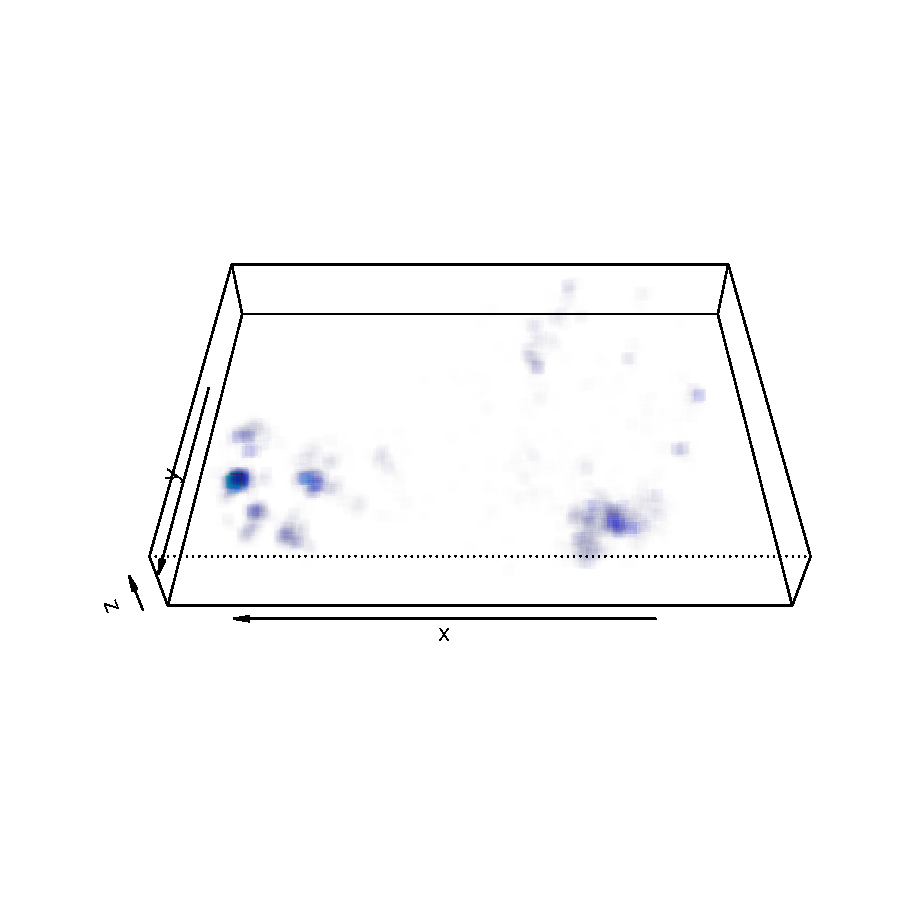
\includegraphics{matter-extra-010}
\caption{\small $m/z$ 5806 (insulin)}
\label{fig:mz5806}
\end{subfigure}
\begin{subfigure}{.4\textwidth}
  \centering
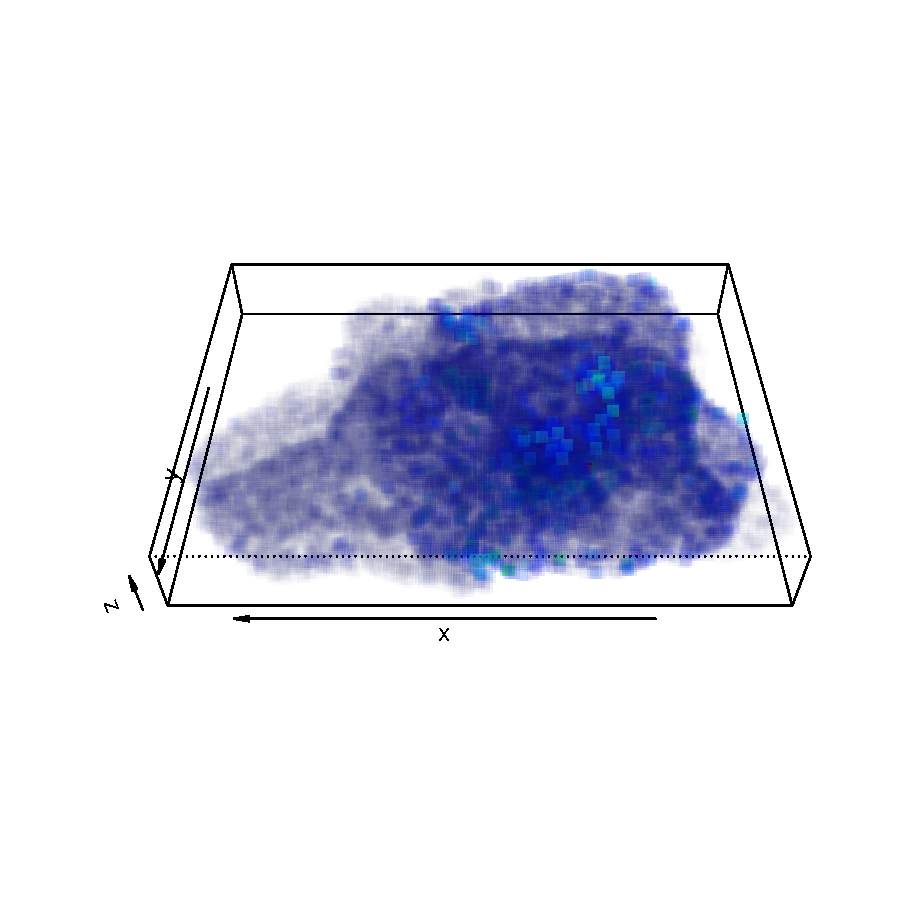
\includegraphics{matter-extra-011}
\caption{\small TIC (total ion current)}
\label{fig:tic}
\end{subfigure}
\caption{\small Plotting 3D images of the benchmark 3D mouse pancreas dataset.}
\end{figure}


\section{Session info}

\begin{itemize}\raggedright
  \item R version 3.3.0 beta (2016-04-19 r70517), \verb|x86_64-apple-darwin13.4.0|
  \item Locale: \verb|en_US.UTF-8/en_US.UTF-8/en_US.UTF-8/C/en_US.UTF-8/en_US.UTF-8|
  \item Base packages: base, datasets, graphics, grDevices, methods, parallel, stats,
    utils
  \item Other packages: biglm~0.9-1, Biobase~2.30.0, BiocGenerics~0.16.1, Cardinal~1.5.0,
    DBI~0.3.1, matter~0.4, ProtGenerics~1.2.1
  \item Loaded via a namespace (and not attached): BiocStyle~1.8.0, grid~3.3.0,
    irlba~2.0.0, lattice~0.20-33, MASS~7.3-45, Matrix~1.2-5, signal~0.7-6, sp~1.2-3,
    stats4~3.3.0, tools~3.3.0
\end{itemize}
% \bibliographystyle{unsrt}
\bibliography{matter-extra}

\end{document}
